\documentclass[twoside]{book}

% Packages required by doxygen
\usepackage{calc}
\usepackage{doxygen}
\usepackage{graphicx}
\usepackage[utf8]{inputenc}
\usepackage{makeidx}
\usepackage{multicol}
\usepackage{multirow}
\usepackage{textcomp}
\usepackage[table]{xcolor}

% Font selection
\usepackage[T1]{fontenc}
\usepackage{mathptmx}
\usepackage[scaled=.90]{helvet}
\usepackage{courier}
\usepackage{amssymb}
\usepackage{sectsty}
\renewcommand{\familydefault}{\sfdefault}
\allsectionsfont{%
  \fontseries{bc}\selectfont%
  \color{darkgray}%
}
\renewcommand{\DoxyLabelFont}{%
  \fontseries{bc}\selectfont%
  \color{darkgray}%
}

% Page & text layout
\usepackage{geometry}
\geometry{%
  a4paper,%
  top=2.5cm,%
  bottom=2.5cm,%
  left=2.5cm,%
  right=2.5cm%
}
\tolerance=750
\hfuzz=15pt
\hbadness=750
\setlength{\emergencystretch}{15pt}
\setlength{\parindent}{0cm}
\setlength{\parskip}{0.2cm}
\makeatletter
\renewcommand{\paragraph}{%
  \@startsection{paragraph}{4}{0ex}{-1.0ex}{1.0ex}{%
    \normalfont\normalsize\bfseries\SS@parafont%
  }%
}
\renewcommand{\subparagraph}{%
  \@startsection{subparagraph}{5}{0ex}{-1.0ex}{1.0ex}{%
    \normalfont\normalsize\bfseries\SS@subparafont%
  }%
}
\makeatother

% Headers & footers
\usepackage{fancyhdr}
\pagestyle{fancyplain}
\fancyhead[LE]{\fancyplain{}{\bfseries\thepage}}
\fancyhead[CE]{\fancyplain{}{}}
\fancyhead[RE]{\fancyplain{}{\bfseries\leftmark}}
\fancyhead[LO]{\fancyplain{}{\bfseries\rightmark}}
\fancyhead[CO]{\fancyplain{}{}}
\fancyhead[RO]{\fancyplain{}{\bfseries\thepage}}
\fancyfoot[LE]{\fancyplain{}{}}
\fancyfoot[CE]{\fancyplain{}{}}
\fancyfoot[RE]{\fancyplain{}{\bfseries\scriptsize Generated on Wed Jan 1 2014 16\-:42\-:37 for Raspboop by Doxygen }}
\fancyfoot[LO]{\fancyplain{}{\bfseries\scriptsize Generated on Wed Jan 1 2014 16\-:42\-:37 for Raspboop by Doxygen }}
\fancyfoot[CO]{\fancyplain{}{}}
\fancyfoot[RO]{\fancyplain{}{}}
\renewcommand{\footrulewidth}{0.4pt}
\renewcommand{\chaptermark}[1]{%
  \markboth{#1}{}%
}
\renewcommand{\sectionmark}[1]{%
  \markright{\thesection\ #1}%
}

% Indices & bibliography
\usepackage{natbib}
\usepackage[titles]{tocloft}
\setcounter{tocdepth}{3}
\setcounter{secnumdepth}{5}
\makeindex

% Hyperlinks (required, but should be loaded last)
\usepackage{ifpdf}
\ifpdf
  \usepackage[pdftex,pagebackref=true]{hyperref}
\else
  \usepackage[ps2pdf,pagebackref=true]{hyperref}
\fi
\hypersetup{%
  colorlinks=true,%
  linkcolor=blue,%
  citecolor=blue,%
  unicode%
}

% Custom commands
\newcommand{\clearemptydoublepage}{%
  \newpage{\pagestyle{empty}\cleardoublepage}%
}


%===== C O N T E N T S =====

\begin{document}

% Titlepage & ToC
\hypersetup{pageanchor=false}
\pagenumbering{roman}
\begin{titlepage}
\vspace*{7cm}
\begin{center}%
{\Large Raspboop \\[1ex]\large 0 }\\
\vspace*{1cm}
{\large Generated by Doxygen 1.8.6}\\
\vspace*{0.5cm}
{\small Wed Jan 1 2014 16:42:37}\\
\end{center}
\end{titlepage}
\clearemptydoublepage
\tableofcontents
\clearemptydoublepage
\pagenumbering{arabic}
\hypersetup{pageanchor=true}

%--- Begin generated contents ---
\chapter{Hierarchical Index}
\section{Class Hierarchy}
This inheritance list is sorted roughly, but not completely, alphabetically\+:\begin{DoxyCompactList}
\item \contentsline{section}{rbp\+:\+:B\+C\+M\+Pins\+P5}{\pageref{classrbp_1_1BCMPinsP5}}{}
\item \contentsline{section}{rbp\+:\+:B\+C\+M\+Pins\+Rev1}{\pageref{classrbp_1_1BCMPinsRev1}}{}
\item \contentsline{section}{rbp\+:\+:B\+C\+M\+Pins\+Rev2}{\pageref{classrbp_1_1BCMPinsRev2}}{}
\item \contentsline{section}{rbp\+:\+:Command}{\pageref{classrbp_1_1Command}}{}
\item \contentsline{section}{rbp\+:\+:Commandable}{\pageref{classrbp_1_1Commandable}}{}
\begin{DoxyCompactList}
\item \contentsline{section}{rbp\+:\+:G\+P\+I\+O\+Consumer}{\pageref{classrbp_1_1GPIOConsumer}}{}
\begin{DoxyCompactList}
\item \contentsline{section}{rbp\+:\+:L298\+N}{\pageref{classrbp_1_1L298N}}{}
\item \contentsline{section}{rbp\+:\+:Sensor}{\pageref{classrbp_1_1Sensor}}{}
\begin{DoxyCompactList}
\item \contentsline{section}{rbp\+:\+:H\+C\+S\+R04}{\pageref{classrbp_1_1HCSR04}}{}
\item \contentsline{section}{rbp\+:\+:H\+C\+S\+R501}{\pageref{classrbp_1_1HCSR501}}{}
\end{DoxyCompactList}
\end{DoxyCompactList}
\end{DoxyCompactList}
\item Q\+Dialog\begin{DoxyCompactList}
\item \contentsline{section}{Robot\+Connect\+Dialog}{\pageref{classRobotConnectDialog}}{}
\end{DoxyCompactList}
\item Q\+Main\+Window\begin{DoxyCompactList}
\item \contentsline{section}{Station\+Window}{\pageref{classStationWindow}}{}
\end{DoxyCompactList}
\item \contentsline{section}{qt\+\_\+meta\+\_\+stringdata\+\_\+\+Robot\+Connect\+Dialog\+\_\+t}{\pageref{structqt__meta__stringdata__RobotConnectDialog__t}}{}
\item \contentsline{section}{qt\+\_\+meta\+\_\+stringdata\+\_\+\+Station\+Window\+\_\+t}{\pageref{structqt__meta__stringdata__StationWindow__t}}{}
\item \contentsline{section}{rbp\+:\+:Serializable}{\pageref{classrbp_1_1Serializable}}{}
\begin{DoxyCompactList}
\item \contentsline{section}{rbp\+:\+:G\+P\+I\+O\+Consumer}{\pageref{classrbp_1_1GPIOConsumer}}{}
\item \contentsline{section}{rbp\+:\+:Server\+:\+:Server\+Quick\+Response\+Code}{\pageref{classrbp_1_1Server_1_1ServerQuickResponseCode}}{}
\end{DoxyCompactList}
\item \contentsline{section}{rbp\+:\+:Server}{\pageref{classrbp_1_1Server}}{}
\item \contentsline{section}{Ui\+\_\+\+Robot\+Connect\+Dialog}{\pageref{classUi__RobotConnectDialog}}{}
\begin{DoxyCompactList}
\item \contentsline{section}{Ui\+:\+:Robot\+Connect\+Dialog}{\pageref{classUi_1_1RobotConnectDialog}}{}
\end{DoxyCompactList}
\item \contentsline{section}{Ui\+\_\+\+Station\+Window}{\pageref{classUi__StationWindow}}{}
\begin{DoxyCompactList}
\item \contentsline{section}{Ui\+:\+:Station\+Window}{\pageref{classUi_1_1StationWindow}}{}
\end{DoxyCompactList}
\item \contentsline{section}{rbp\+:\+:Wiring\+Pi\+Pins}{\pageref{classrbp_1_1WiringPiPins}}{}
\item \contentsline{section}{rbp\+:\+:Wiring\+Pi\+Pins\+P5}{\pageref{classrbp_1_1WiringPiPinsP5}}{}
\end{DoxyCompactList}

\chapter{Class Index}
\section{Class List}
Here are the classes, structs, unions and interfaces with brief descriptions\+:\begin{DoxyCompactList}
\item\contentsline{section}{\hyperlink{classrbp_1_1BCMPinsP5}{rbp\+::\+B\+C\+M\+Pins\+P5} \\*Convenience class for the P5 connector on the Raspberry Pi Model B This class is specific to the B\+C\+M G\+P\+I\+O pin numbering \href{http://wiringpi.com/pins/}{\tt Pin reference} }{\pageref{classrbp_1_1BCMPinsP5}}{}
\item\contentsline{section}{\hyperlink{classrbp_1_1BCMPinsRev1}{rbp\+::\+B\+C\+M\+Pins\+Rev1} \\*A B\+C\+M G\+P\+I\+O convenience class for Revision 1/model A Raspberry Pi\textquotesingle{}s \href{http://wiringpi.com/pins/}{\tt Pin reference} }{\pageref{classrbp_1_1BCMPinsRev1}}{}
\item\contentsline{section}{\hyperlink{classrbp_1_1BCMPinsRev2}{rbp\+::\+B\+C\+M\+Pins\+Rev2} \\*A B\+C\+M G\+P\+I\+O convenience class for Revision 2/model B Raspberry Pi\textquotesingle{}s \href{http://wiringpi.com/pins/}{\tt Pin reference} }{\pageref{classrbp_1_1BCMPinsRev2}}{}
\item\contentsline{section}{\hyperlink{classrbp_1_1Command}{rbp\+::\+Command} \\*Encapsulates data into a command }{\pageref{classrbp_1_1Command}}{}
\item\contentsline{section}{\hyperlink{classrbp_1_1Commandable}{rbp\+::\+Commandable} \\*Interface for objects that can accept Commands }{\pageref{classrbp_1_1Commandable}}{}
\item\contentsline{section}{\hyperlink{classrbp_1_1GPIOConsumer}{rbp\+::\+G\+P\+I\+O\+Consumer} \\*Abstract class for all G\+P\+I\+O pin utilizers }{\pageref{classrbp_1_1GPIOConsumer}}{}
\item\contentsline{section}{\hyperlink{classrbp_1_1HCSR04}{rbp\+::\+H\+C\+S\+R04} \\*Ultrasonic distance sensor }{\pageref{classrbp_1_1HCSR04}}{}
\item\contentsline{section}{\hyperlink{classrbp_1_1HCSR501}{rbp\+::\+H\+C\+S\+R501} \\*Passive infrared sensor for motion detection }{\pageref{classrbp_1_1HCSR501}}{}
\item\contentsline{section}{\hyperlink{classrbp_1_1L298N}{rbp\+::\+L298\+N} \\*\hyperlink{classrbp_1_1L298N}{L298\+N} Motor controller }{\pageref{classrbp_1_1L298N}}{}
\item\contentsline{section}{\hyperlink{structqt__meta__stringdata__RobotConnectDialog__t}{qt\+\_\+meta\+\_\+stringdata\+\_\+\+Robot\+Connect\+Dialog\+\_\+t} }{\pageref{structqt__meta__stringdata__RobotConnectDialog__t}}{}
\item\contentsline{section}{\hyperlink{structqt__meta__stringdata__StationWindow__t}{qt\+\_\+meta\+\_\+stringdata\+\_\+\+Station\+Window\+\_\+t} }{\pageref{structqt__meta__stringdata__StationWindow__t}}{}
\item\contentsline{section}{\hyperlink{classUi_1_1RobotConnectDialog}{Ui\+::\+Robot\+Connect\+Dialog} }{\pageref{classUi_1_1RobotConnectDialog}}{}
\item\contentsline{section}{\hyperlink{classRobotConnectDialog}{Robot\+Connect\+Dialog} }{\pageref{classRobotConnectDialog}}{}
\item\contentsline{section}{\hyperlink{classrbp_1_1Sensor}{rbp\+::\+Sensor} \\*An abstract class for devices that can interface with the world }{\pageref{classrbp_1_1Sensor}}{}
\item\contentsline{section}{\hyperlink{classrbp_1_1Serializable}{rbp\+::\+Serializable} \\*Interface for objects that can be serialized }{\pageref{classrbp_1_1Serializable}}{}
\item\contentsline{section}{\hyperlink{classrbp_1_1Server}{rbp\+::\+Server} \\*\hyperlink{classrbp_1_1Server}{Server} class used to receive Commands }{\pageref{classrbp_1_1Server}}{}
\item\contentsline{section}{\hyperlink{classrbp_1_1Server_1_1ServerQuickResponseCode}{rbp\+::\+Server\+::\+Server\+Quick\+Response\+Code} \\*A convenience class used to quickly send a response code }{\pageref{classrbp_1_1Server_1_1ServerQuickResponseCode}}{}
\item\contentsline{section}{\hyperlink{classStationWindow}{Station\+Window} }{\pageref{classStationWindow}}{}
\item\contentsline{section}{\hyperlink{classUi_1_1StationWindow}{Ui\+::\+Station\+Window} }{\pageref{classUi_1_1StationWindow}}{}
\item\contentsline{section}{\hyperlink{classUi__RobotConnectDialog}{Ui\+\_\+\+Robot\+Connect\+Dialog} }{\pageref{classUi__RobotConnectDialog}}{}
\item\contentsline{section}{\hyperlink{classUi__StationWindow}{Ui\+\_\+\+Station\+Window} }{\pageref{classUi__StationWindow}}{}
\item\contentsline{section}{\hyperlink{classrbp_1_1WiringPiPins}{rbp\+::\+Wiring\+Pi\+Pins} \\*A convenience class for the P1 G\+P\+I\+O Connector pins \href{http://wiringpi.com/pins/}{\tt Pin reference} }{\pageref{classrbp_1_1WiringPiPins}}{}
\item\contentsline{section}{\hyperlink{classrbp_1_1WiringPiPinsP5}{rbp\+::\+Wiring\+Pi\+Pins\+P5} \\*A convenience class for the P5 connector on the Raspberry Pi Model B This class is specific to the Wiring\+Pi pin numbering \href{http://wiringpi.com/pins/}{\tt Pin reference} }{\pageref{classrbp_1_1WiringPiPinsP5}}{}
\end{DoxyCompactList}

\chapter{Class Documentation}
\hypertarget{classraspboop_1_1GPIOConsumer}{\section{raspboop\-:\-:G\-P\-I\-O\-Consumer Class Reference}
\label{classraspboop_1_1GPIOConsumer}\index{raspboop\-::\-G\-P\-I\-O\-Consumer@{raspboop\-::\-G\-P\-I\-O\-Consumer}}
}


Abstract class for all G\-P\-I\-O pin utilizers.  




{\ttfamily \#include $<$G\-P\-I\-O\-Consumer.\-h$>$}

Inheritance diagram for raspboop\-:\-:G\-P\-I\-O\-Consumer\-:\begin{figure}[H]
\begin{center}
\leavevmode
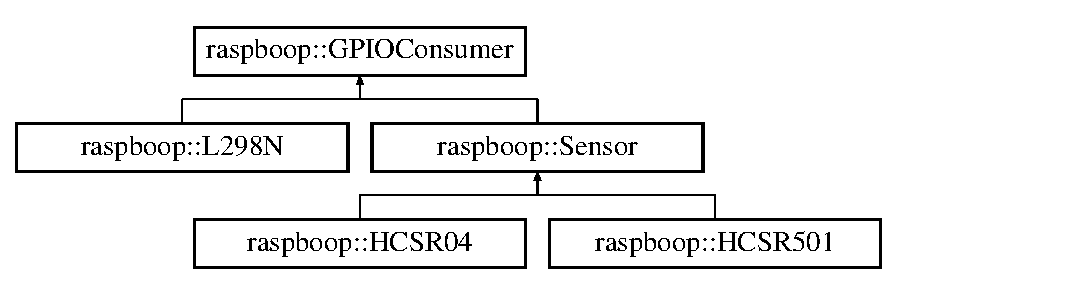
\includegraphics[height=3.000000cm]{classraspboop_1_1GPIOConsumer}
\end{center}
\end{figure}
\subsection*{Protected Member Functions}
\begin{DoxyCompactItemize}
\item 
void \hyperlink{classraspboop_1_1GPIOConsumer_a066938a39a4f34ed2cfee05a593008e6}{Consume\-Pin} (int Pin, int Mode) const 
\begin{DoxyCompactList}\small\item\em Reserves a pin and sets its mode. \end{DoxyCompactList}\item 
virtual void \hyperlink{classraspboop_1_1GPIOConsumer_a97b06b9afddfb338fb87cb7338c910de}{Release\-Pins} ()=0
\begin{DoxyCompactList}\small\item\em Sets the mode of all pins to an inactive state. \end{DoxyCompactList}\end{DoxyCompactItemize}


\subsection{Detailed Description}
Abstract class for all G\-P\-I\-O pin utilizers. 

If a class will interface with the Raspberry Pi's G\-P\-I\-O pins, then it must inherit from this class. This is to ensure that all children will be forced to use the {\ttfamily \hyperlink{classraspboop_1_1GPIOConsumer_a97b06b9afddfb338fb87cb7338c910de}{Release\-Pins()}} method, which sets the value of any active pins to an inactive state.

Also, the {\ttfamily \hyperlink{classraspboop_1_1GPIOConsumer_a066938a39a4f34ed2cfee05a593008e6}{Consume\-Pin()}} method provides a layer of abstraction over the wiring\-Pi {\ttfamily pin\-Mode()} method. In the future, this method will be a friend of the \hyperlink{classraspboop_1_1GPIOManager}{G\-P\-I\-O\-Manager} class. 

\subsection{Member Function Documentation}
\hypertarget{classraspboop_1_1GPIOConsumer_a066938a39a4f34ed2cfee05a593008e6}{\index{raspboop\-::\-G\-P\-I\-O\-Consumer@{raspboop\-::\-G\-P\-I\-O\-Consumer}!Consume\-Pin@{Consume\-Pin}}
\index{Consume\-Pin@{Consume\-Pin}!raspboop::GPIOConsumer@{raspboop\-::\-G\-P\-I\-O\-Consumer}}
\subsubsection[{Consume\-Pin}]{\setlength{\rightskip}{0pt plus 5cm}void raspboop\-::\-G\-P\-I\-O\-Consumer\-::\-Consume\-Pin (
\begin{DoxyParamCaption}
\item[{int}]{Pin, }
\item[{int}]{Mode}
\end{DoxyParamCaption}
) const\hspace{0.3cm}{\ttfamily [protected]}}}\label{classraspboop_1_1GPIOConsumer_a066938a39a4f34ed2cfee05a593008e6}


Reserves a pin and sets its mode. 

Uses wiring\-Pi's {\itshape pin\-Mode()} method to set the value of the {\itshape Pin} to the {\itshape Mode} parameter.


\begin{DoxyParams}{Parameters}
{\em Pin} & the G\-P\-I\-O pin to set \\
\hline
{\em Mode} & The Mode the Pin will be set to \\
\hline
\end{DoxyParams}
\hypertarget{classraspboop_1_1GPIOConsumer_a97b06b9afddfb338fb87cb7338c910de}{\index{raspboop\-::\-G\-P\-I\-O\-Consumer@{raspboop\-::\-G\-P\-I\-O\-Consumer}!Release\-Pins@{Release\-Pins}}
\index{Release\-Pins@{Release\-Pins}!raspboop::GPIOConsumer@{raspboop\-::\-G\-P\-I\-O\-Consumer}}
\subsubsection[{Release\-Pins}]{\setlength{\rightskip}{0pt plus 5cm}virtual void raspboop\-::\-G\-P\-I\-O\-Consumer\-::\-Release\-Pins (
\begin{DoxyParamCaption}
{}
\end{DoxyParamCaption}
)\hspace{0.3cm}{\ttfamily [protected]}, {\ttfamily [pure virtual]}}}\label{classraspboop_1_1GPIOConsumer_a97b06b9afddfb338fb87cb7338c910de}


Sets the mode of all pins to an inactive state. 

All children must call this method when it becomes out of scope, preferably in the destructor. This is necessary so that there are never any G\-P\-I\-O pins unnecessarily set to {\itshape H\-I\-G\-H} 

Implemented in \hyperlink{classraspboop_1_1HCSR04_a194e41e6234c6c81bb9b022dc16b98ac}{raspboop\-::\-H\-C\-S\-R04}, \hyperlink{classraspboop_1_1L298N_a5ed5847ed8db5835fbf5e4f960a374e9}{raspboop\-::\-L298\-N}, and \hyperlink{classraspboop_1_1HCSR501_aa8609b3c9529ff3863d47010fc9e78d0}{raspboop\-::\-H\-C\-S\-R501}.



The documentation for this class was generated from the following files\-:\begin{DoxyCompactItemize}
\item 
include/raspboop/abstracts/G\-P\-I\-O\-Consumer.\-h\item 
src/abstracts/G\-P\-I\-O\-Consumer.\-cpp\end{DoxyCompactItemize}

\hypertarget{classraspboop_1_1GPIOManager}{\section{raspboop\-:\-:G\-P\-I\-O\-Manager Class Reference}
\label{classraspboop_1_1GPIOManager}\index{raspboop\-::\-G\-P\-I\-O\-Manager@{raspboop\-::\-G\-P\-I\-O\-Manager}}
}


Manages the use of G\-P\-I\-O pins. {\bfseries Unimplemented}  




{\ttfamily \#include $<$G\-P\-I\-O\-Manager.\-h$>$}

\subsection*{Public Member Functions}
\begin{DoxyCompactItemize}
\item 
\hypertarget{classraspboop_1_1GPIOManager_a5ed2a83f4b2629e8eda38f1ed48679f4}{int {\bfseries Is\-Pin\-Set} (int Pin)}\label{classraspboop_1_1GPIOManager_a5ed2a83f4b2629e8eda38f1ed48679f4}

\end{DoxyCompactItemize}


\subsection{Detailed Description}
Manages the use of G\-P\-I\-O pins. {\bfseries Unimplemented} 

This class is not finished. 

The documentation for this class was generated from the following files\-:\begin{DoxyCompactItemize}
\item 
include/raspboop/controls/G\-P\-I\-O\-Manager.\-h\item 
src/controls/G\-P\-I\-O\-Manager.\-cpp\end{DoxyCompactItemize}

\hypertarget{classraspboop_1_1HCSR04}{\section{raspboop\-:\-:H\-C\-S\-R04 Class Reference}
\label{classraspboop_1_1HCSR04}\index{raspboop\-::\-H\-C\-S\-R04@{raspboop\-::\-H\-C\-S\-R04}}
}


Ultrasonic distance sensor.  




{\ttfamily \#include $<$H\-C\-S\-R04.\-h$>$}

Inheritance diagram for raspboop\-:\-:H\-C\-S\-R04\-:\begin{figure}[H]
\begin{center}
\leavevmode
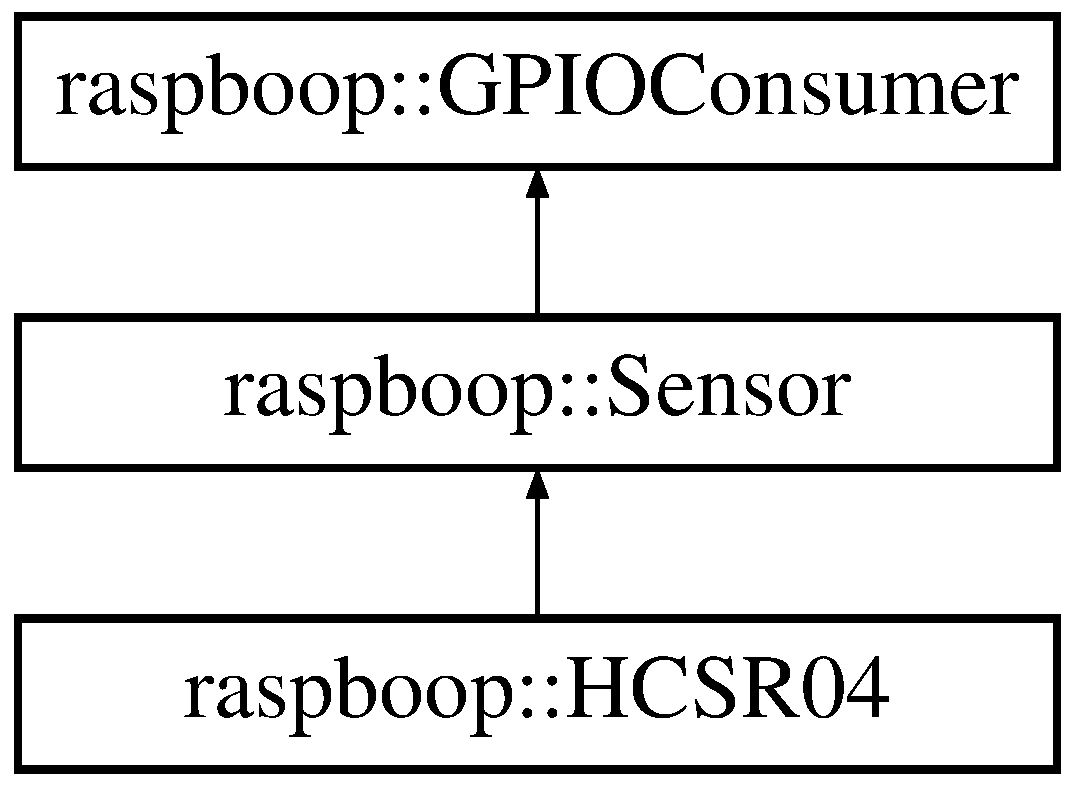
\includegraphics[height=3.000000cm]{classraspboop_1_1HCSR04}
\end{center}
\end{figure}
\subsection*{Public Member Functions}
\begin{DoxyCompactItemize}
\item 
virtual void \hyperlink{classraspboop_1_1HCSR04_ab25ac4ca02a3a3e3b00d0df95c58f447}{Sense} ()
\begin{DoxyCompactList}\small\item\em Performs the sensor's sensing operation. \end{DoxyCompactList}\item 
float \hyperlink{classraspboop_1_1HCSR04_ad242d219ab8b6adbf1d684416ba47cb9}{Get\-Distance} () const 
\begin{DoxyCompactList}\small\item\em Get the distance calculated from the sensor. \end{DoxyCompactList}\item 
\hypertarget{classraspboop_1_1HCSR04_af82593e779415b2ec0b5820f45901187}{\hyperlink{classraspboop_1_1HCSR04_af82593e779415b2ec0b5820f45901187}{$\sim$\-H\-C\-S\-R04} ()}\label{classraspboop_1_1HCSR04_af82593e779415b2ec0b5820f45901187}

\begin{DoxyCompactList}\small\item\em \hyperlink{classraspboop_1_1HCSR04}{H\-C\-S\-R04} Destructor. \end{DoxyCompactList}\end{DoxyCompactItemize}
\subsection*{Static Public Member Functions}
\begin{DoxyCompactItemize}
\item 
static \hyperlink{classraspboop_1_1HCSR04}{H\-C\-S\-R04} $\ast$ \hyperlink{classraspboop_1_1HCSR04_a7e89b5599fc715d1c903ff69f8aa2665}{Create} (int E\-C\-H\-O, int T\-R\-I\-G)
\begin{DoxyCompactList}\small\item\em Create a usable \hyperlink{classraspboop_1_1HCSR04}{H\-C\-S\-R04} object. \end{DoxyCompactList}\end{DoxyCompactItemize}
\subsection*{Protected Member Functions}
\begin{DoxyCompactItemize}
\item 
virtual void \hyperlink{classraspboop_1_1HCSR04_a194e41e6234c6c81bb9b022dc16b98ac}{Release\-Pins} ()
\begin{DoxyCompactList}\small\item\em Sets the mode of all pins to an inactive state. \end{DoxyCompactList}\end{DoxyCompactItemize}


\subsection{Detailed Description}
Ultrasonic distance sensor. 

The \hyperlink{classraspboop_1_1HCSR04}{H\-C\-S\-R04} is an ultrasonic distance sensor. By emitting an ultrasonic sound, the distance between the sensor and another object can be calculated through the formula\-:

d = t $\ast$ 340 /2

where, {\itshape d} is distance in meters, {\itshape t} is time in seconds, {\itshape 340} is the speed of sound in m/s

We divide by two because the sound had to travel back to the sensor.

\subsection*{Helpful information }


\begin{DoxyItemize}
\item The sensor has 4 pins
\begin{DoxyItemize}
\item {\bfseries Vcc} input 5\-V here
\item {\bfseries Trig} Input used to tell the sensor when to send the sound
\item {\bfseries Echo} The output from the sensor
\item {\bfseries G\-N\-D} Connect this to ground
\end{DoxyItemize}
\end{DoxyItemize}

{\bfseries I\-M\-P\-O\-R\-T\-A\-N\-T I\-N\-F\-O\-R\-M\-A\-T\-I\-O\-N\-:} The Raspberry Pi's pins operate at 3\-V3 volt logic. This means that you must use a voltage divider on the Echo pin when reading in a value. I recommend using two resistors whose values are 1.\-5x apart. For more detailed instructions on how to do this, visit\-: \href{http://www.bytecreation.com/blog/2013/10/13/
 raspberry-pi-ultrasonic-sensor-hc-sr04}{\tt bytecreation.\-com}

\begin{TabularC}{2}
\hline
\rowcolor{lightgray}{\bf Quick Stats }&{\bf Value  }\\\cline{1-2}
Operating Voltage &{\bfseries 5\-V} \\\cline{1-2}
Operating Current &{\bfseries 15 m\-A} \\\cline{1-2}
Soundwave frequency &{\bfseries 40 Hz} \\\cline{1-2}
Maximum distance &{\bfseries 4m} \\\cline{1-2}
Minimum distance &{\bfseries 2 cm} \\\cline{1-2}
Required Trigger pulse &{\bfseries 10us (microseconds) H\-I\-G\-H signal} \\\cline{1-2}
\end{TabularC}


\subsubsection*{External links }

\href{http://users.ece.utexas.edu/~valvano/Datasheets/
HCSR04b.pdf}{\tt Datasheet}

\href{http://www.bytecreation.com/blog/2013/10/13/
raspberry-pi-ultrasonic-sensor-hc-sr04}{\tt Blog post\-:} Good article that details the steps necessary to use this sensor with a raspberry pi and a voltage divider. 

\subsection{Member Function Documentation}
\hypertarget{classraspboop_1_1HCSR04_a7e89b5599fc715d1c903ff69f8aa2665}{\index{raspboop\-::\-H\-C\-S\-R04@{raspboop\-::\-H\-C\-S\-R04}!Create@{Create}}
\index{Create@{Create}!raspboop::HCSR04@{raspboop\-::\-H\-C\-S\-R04}}
\subsubsection[{Create}]{\setlength{\rightskip}{0pt plus 5cm}{\bf H\-C\-S\-R04} $\ast$ raspboop\-::\-H\-C\-S\-R04\-::\-Create (
\begin{DoxyParamCaption}
\item[{int}]{E\-C\-H\-O, }
\item[{int}]{T\-R\-I\-G}
\end{DoxyParamCaption}
)\hspace{0.3cm}{\ttfamily [static]}}}\label{classraspboop_1_1HCSR04_a7e89b5599fc715d1c903ff69f8aa2665}


Create a usable \hyperlink{classraspboop_1_1HCSR04}{H\-C\-S\-R04} object. 

To properly create an object in raspboop, you must use its factory \hyperlink{classraspboop_1_1HCSR04_a7e89b5599fc715d1c903ff69f8aa2665}{Create()} method. The factory method initializes the \hyperlink{classraspboop_1_1HCSR04}{H\-C\-S\-R04}'s pins using the \hyperlink{classraspboop_1_1Sensor_ad0b3f0fa153803108613e3c3da574571}{Set\-Input\-Pin()} and \hyperlink{classraspboop_1_1Sensor_a893f7ad09018028fdb9e10f0bcbeccf9}{Set\-Output\-Pin()} methods inherited from \hyperlink{classraspboop_1_1Sensor}{Sensor}.


\begin{DoxyParams}{Parameters}
{\em E\-C\-H\-O} & The input pin designated to read the sensors E\-C\-H\-O output \\
\hline
{\em T\-R\-I\-G} & The output pin that initiates sensing\\
\hline
\end{DoxyParams}
\begin{DoxyReturn}{Returns}
A pointer to an \hyperlink{classraspboop_1_1HCSR04}{H\-C\-S\-R04} object with all pins initialized 
\end{DoxyReturn}
\hypertarget{classraspboop_1_1HCSR04_ad242d219ab8b6adbf1d684416ba47cb9}{\index{raspboop\-::\-H\-C\-S\-R04@{raspboop\-::\-H\-C\-S\-R04}!Get\-Distance@{Get\-Distance}}
\index{Get\-Distance@{Get\-Distance}!raspboop::HCSR04@{raspboop\-::\-H\-C\-S\-R04}}
\subsubsection[{Get\-Distance}]{\setlength{\rightskip}{0pt plus 5cm}float raspboop\-::\-H\-C\-S\-R04\-::\-Get\-Distance (
\begin{DoxyParamCaption}
{}
\end{DoxyParamCaption}
) const\hspace{0.3cm}{\ttfamily [inline]}}}\label{classraspboop_1_1HCSR04_ad242d219ab8b6adbf1d684416ba47cb9}


Get the distance calculated from the sensor. 

\begin{DoxyReturn}{Returns}
A float representing the distance sensed in centimeters 
\end{DoxyReturn}
\hypertarget{classraspboop_1_1HCSR04_a194e41e6234c6c81bb9b022dc16b98ac}{\index{raspboop\-::\-H\-C\-S\-R04@{raspboop\-::\-H\-C\-S\-R04}!Release\-Pins@{Release\-Pins}}
\index{Release\-Pins@{Release\-Pins}!raspboop::HCSR04@{raspboop\-::\-H\-C\-S\-R04}}
\subsubsection[{Release\-Pins}]{\setlength{\rightskip}{0pt plus 5cm}void raspboop\-::\-H\-C\-S\-R04\-::\-Release\-Pins (
\begin{DoxyParamCaption}
{}
\end{DoxyParamCaption}
)\hspace{0.3cm}{\ttfamily [protected]}, {\ttfamily [virtual]}}}\label{classraspboop_1_1HCSR04_a194e41e6234c6c81bb9b022dc16b98ac}


Sets the mode of all pins to an inactive state. 

All children must call this method when it becomes out of scope, preferably in the destructor. This is necessary so that there are never any G\-P\-I\-O pins unnecessarily set to {\itshape H\-I\-G\-H} 

Implements \hyperlink{classraspboop_1_1GPIOConsumer_a97b06b9afddfb338fb87cb7338c910de}{raspboop\-::\-G\-P\-I\-O\-Consumer}.

\hypertarget{classraspboop_1_1HCSR04_ab25ac4ca02a3a3e3b00d0df95c58f447}{\index{raspboop\-::\-H\-C\-S\-R04@{raspboop\-::\-H\-C\-S\-R04}!Sense@{Sense}}
\index{Sense@{Sense}!raspboop::HCSR04@{raspboop\-::\-H\-C\-S\-R04}}
\subsubsection[{Sense}]{\setlength{\rightskip}{0pt plus 5cm}void raspboop\-::\-H\-C\-S\-R04\-::\-Sense (
\begin{DoxyParamCaption}
{}
\end{DoxyParamCaption}
)\hspace{0.3cm}{\ttfamily [virtual]}}}\label{classraspboop_1_1HCSR04_ab25ac4ca02a3a3e3b00d0df95c58f447}


Performs the sensor's sensing operation. 

This method will retrieve a value from the environment by performing G\-P\-I\-O operations on the input and output pins of the sensor. The value from the sensor will be available through an accessor method. 

Implements \hyperlink{classraspboop_1_1Sensor_ab854a10682373803a310c078bb71aacf}{raspboop\-::\-Sensor}.



The documentation for this class was generated from the following files\-:\begin{DoxyCompactItemize}
\item 
include/raspboop/sensors/H\-C\-S\-R04.\-h\item 
src/sensors/H\-C\-S\-R04.\-cpp\end{DoxyCompactItemize}

\hypertarget{classraspboop_1_1HCSR501}{\section{raspboop\-:\-:H\-C\-S\-R501 Class Reference}
\label{classraspboop_1_1HCSR501}\index{raspboop\-::\-H\-C\-S\-R501@{raspboop\-::\-H\-C\-S\-R501}}
}


Passive infrared sensor for motion detection.  




{\ttfamily \#include $<$H\-C\-S\-R501.\-h$>$}

Inheritance diagram for raspboop\-:\-:H\-C\-S\-R501\-:\begin{figure}[H]
\begin{center}
\leavevmode
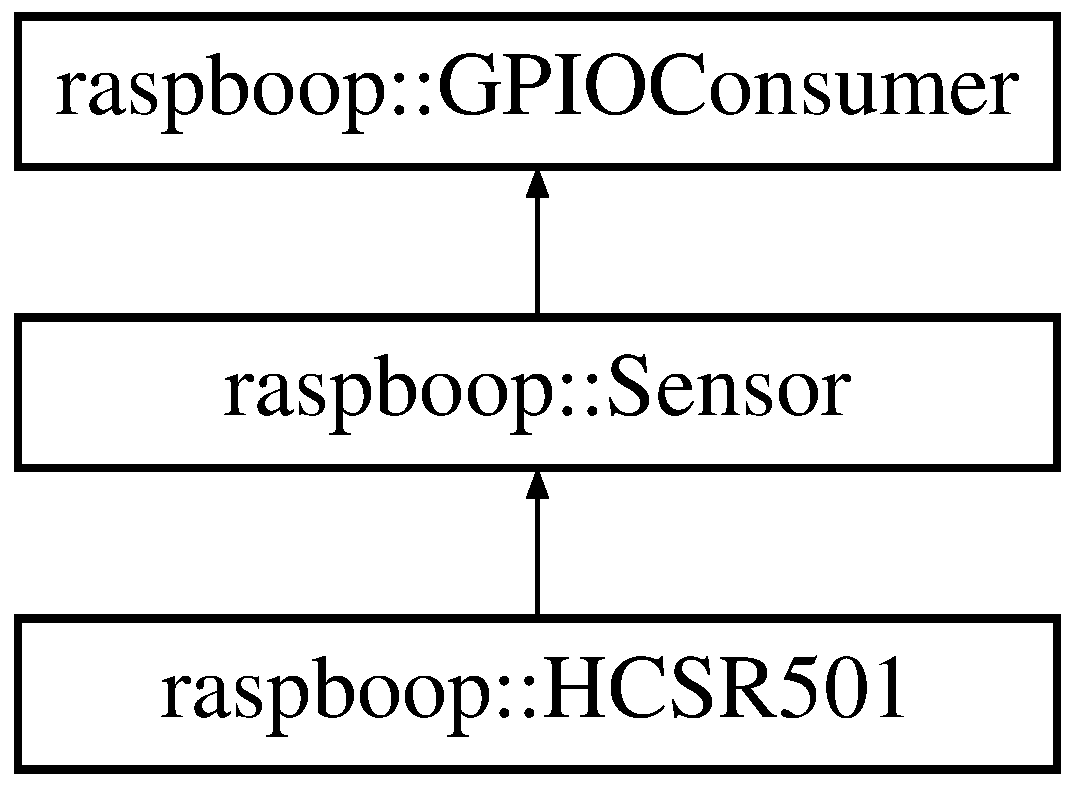
\includegraphics[height=3.000000cm]{classraspboop_1_1HCSR501}
\end{center}
\end{figure}
\subsection*{Public Member Functions}
\begin{DoxyCompactItemize}
\item 
\hyperlink{classraspboop_1_1HCSR501_aeb198c632522d10e5319184ac85c303e}{H\-C\-S\-R501} ()
\begin{DoxyCompactList}\small\item\em \hyperlink{classraspboop_1_1HCSR501}{H\-C\-S\-R501} Constructor. \end{DoxyCompactList}\item 
virtual void \hyperlink{classraspboop_1_1HCSR501_ade0ae21c1bda3dabec68e0476d92520a}{Sense} ()
\begin{DoxyCompactList}\small\item\em Performs the sensor's sensing operation. \end{DoxyCompactList}\item 
bool \hyperlink{classraspboop_1_1HCSR501_a06f7b6c117ee5acf76592a3f89159a3e}{Is\-Signalled} () const 
\begin{DoxyCompactList}\small\item\em Get the value obtained from \hyperlink{classraspboop_1_1HCSR501_ade0ae21c1bda3dabec68e0476d92520a}{Sense()} \end{DoxyCompactList}\item 
\hypertarget{classraspboop_1_1HCSR501_a8a25051cf0c8ae1700b933419749366d}{\hyperlink{classraspboop_1_1HCSR501_a8a25051cf0c8ae1700b933419749366d}{$\sim$\-H\-C\-S\-R501} ()}\label{classraspboop_1_1HCSR501_a8a25051cf0c8ae1700b933419749366d}

\begin{DoxyCompactList}\small\item\em \hyperlink{classraspboop_1_1HCSR501}{H\-C\-S\-R501} destructor. \end{DoxyCompactList}\end{DoxyCompactItemize}
\subsection*{Static Public Member Functions}
\begin{DoxyCompactItemize}
\item 
static \hyperlink{classraspboop_1_1HCSR501}{H\-C\-S\-R501} $\ast$ \hyperlink{classraspboop_1_1HCSR501_ad2a07d3f130362206c5fbcce92d41294}{Create} (int S\-I\-G\-N\-A\-L)
\begin{DoxyCompactList}\small\item\em Create a usable \hyperlink{classraspboop_1_1HCSR501}{H\-C\-S\-R501} object. \end{DoxyCompactList}\end{DoxyCompactItemize}
\subsection*{Protected Member Functions}
\begin{DoxyCompactItemize}
\item 
virtual void \hyperlink{classraspboop_1_1HCSR501_aa8609b3c9529ff3863d47010fc9e78d0}{Release\-Pins} ()
\begin{DoxyCompactList}\small\item\em Sets the mode of all pins to an inactive state. \end{DoxyCompactList}\end{DoxyCompactItemize}


\subsection{Detailed Description}
Passive infrared sensor for motion detection. 

The \hyperlink{classraspboop_1_1HCSR501}{H\-C\-S\-R501} is a passive infrared sensor used for motion detection applications. There are 5 main pins that you will need to be familiar with\-:


\begin{DoxyItemize}
\item 5\-V input
\item Signal
\item Gnd
\item retriggering pin
\item non-\/retriggering pin
\end{DoxyItemize}

\subsection*{Helpful information }

There are two modes to the sensor\-: retriggering, and non-\/retriggering. In retriggering mode, signal outputs high as long as motion is detected. In non-\/retriggering mode, signal will output as H\-I\-G\-H only every second or so that motion is detected.

\begin{TabularC}{2}
\hline
\rowcolor{lightgray}{\bf Quick Stats }&{\bf Value  }\\\cline{1-2}
Vcc &{\bfseries 5-\/16\-V} \\\cline{1-2}
Logical voltage &{\bfseries 3\-V3} \\\cline{1-2}
Sensing range &{\bfseries 7 meters} \\\cline{1-2}
\end{TabularC}
\subsubsection*{External Links }

\href{http://www.ladyada.net/media/
sensors/PIRSensor-V1.2.pdf}{\tt Parallax P\-I\-R datasheet}

\href{http://elecfreaks.com/store/download/
datasheet/sensor/DYP-ME003/Specification.pdf}{\tt Elec Freaks datasheet}

\href{http://
www.ladyada.net/learn/sensors/pir.html}{\tt P\-I\-R motion sensors tutorial by Lady\-Ada.\-net}

\href{http://robotic-controls.com/learn/sensors/pir-sensor-hc-sr501}{\tt Supplementary Arduino code and tutorial} 

\subsection{Constructor \& Destructor Documentation}
\hypertarget{classraspboop_1_1HCSR501_aeb198c632522d10e5319184ac85c303e}{\index{raspboop\-::\-H\-C\-S\-R501@{raspboop\-::\-H\-C\-S\-R501}!H\-C\-S\-R501@{H\-C\-S\-R501}}
\index{H\-C\-S\-R501@{H\-C\-S\-R501}!raspboop::HCSR501@{raspboop\-::\-H\-C\-S\-R501}}
\subsubsection[{H\-C\-S\-R501}]{\setlength{\rightskip}{0pt plus 5cm}raspboop\-::\-H\-C\-S\-R501\-::\-H\-C\-S\-R501 (
\begin{DoxyParamCaption}
{}
\end{DoxyParamCaption}
)}}\label{classraspboop_1_1HCSR501_aeb198c632522d10e5319184ac85c303e}


\hyperlink{classraspboop_1_1HCSR501}{H\-C\-S\-R501} Constructor. 

Initializes private variables to unused values 

\subsection{Member Function Documentation}
\hypertarget{classraspboop_1_1HCSR501_ad2a07d3f130362206c5fbcce92d41294}{\index{raspboop\-::\-H\-C\-S\-R501@{raspboop\-::\-H\-C\-S\-R501}!Create@{Create}}
\index{Create@{Create}!raspboop::HCSR501@{raspboop\-::\-H\-C\-S\-R501}}
\subsubsection[{Create}]{\setlength{\rightskip}{0pt plus 5cm}{\bf H\-C\-S\-R501} $\ast$ raspboop\-::\-H\-C\-S\-R501\-::\-Create (
\begin{DoxyParamCaption}
\item[{int}]{S\-I\-G\-N\-A\-L}
\end{DoxyParamCaption}
)\hspace{0.3cm}{\ttfamily [static]}}}\label{classraspboop_1_1HCSR501_ad2a07d3f130362206c5fbcce92d41294}


Create a usable \hyperlink{classraspboop_1_1HCSR501}{H\-C\-S\-R501} object. 

To properly create an object in raspboop, you must use its factory \hyperlink{classraspboop_1_1HCSR501_ad2a07d3f130362206c5fbcce92d41294}{Create()} method. The factory method initializes the \hyperlink{classraspboop_1_1HCSR501}{H\-C\-S\-R501}'s Signal pin using the \hyperlink{classraspboop_1_1Sensor_ad0b3f0fa153803108613e3c3da574571}{Set\-Input\-Pin()} method from \hyperlink{classraspboop_1_1Sensor}{Sensor}.


\begin{DoxyParams}{Parameters}
{\em S\-I\-G\-N\-A\-L} & The input pin which will read the value from the sensor\\
\hline
\end{DoxyParams}
\begin{DoxyReturn}{Returns}
A pointer to an \hyperlink{classraspboop_1_1HCSR501}{H\-C\-S\-R501} object with all pins initialized 
\end{DoxyReturn}
\hypertarget{classraspboop_1_1HCSR501_a06f7b6c117ee5acf76592a3f89159a3e}{\index{raspboop\-::\-H\-C\-S\-R501@{raspboop\-::\-H\-C\-S\-R501}!Is\-Signalled@{Is\-Signalled}}
\index{Is\-Signalled@{Is\-Signalled}!raspboop::HCSR501@{raspboop\-::\-H\-C\-S\-R501}}
\subsubsection[{Is\-Signalled}]{\setlength{\rightskip}{0pt plus 5cm}bool raspboop\-::\-H\-C\-S\-R501\-::\-Is\-Signalled (
\begin{DoxyParamCaption}
{}
\end{DoxyParamCaption}
) const\hspace{0.3cm}{\ttfamily [inline]}}}\label{classraspboop_1_1HCSR501_a06f7b6c117ee5acf76592a3f89159a3e}


Get the value obtained from \hyperlink{classraspboop_1_1HCSR501_ade0ae21c1bda3dabec68e0476d92520a}{Sense()} 

\begin{DoxyReturn}{Returns}
A boolean value determining the signal pin's value 
\end{DoxyReturn}
\hypertarget{classraspboop_1_1HCSR501_aa8609b3c9529ff3863d47010fc9e78d0}{\index{raspboop\-::\-H\-C\-S\-R501@{raspboop\-::\-H\-C\-S\-R501}!Release\-Pins@{Release\-Pins}}
\index{Release\-Pins@{Release\-Pins}!raspboop::HCSR501@{raspboop\-::\-H\-C\-S\-R501}}
\subsubsection[{Release\-Pins}]{\setlength{\rightskip}{0pt plus 5cm}void raspboop\-::\-H\-C\-S\-R501\-::\-Release\-Pins (
\begin{DoxyParamCaption}
{}
\end{DoxyParamCaption}
)\hspace{0.3cm}{\ttfamily [protected]}, {\ttfamily [virtual]}}}\label{classraspboop_1_1HCSR501_aa8609b3c9529ff3863d47010fc9e78d0}


Sets the mode of all pins to an inactive state. 

All children must call this method when it becomes out of scope, preferably in the destructor. This is necessary so that there are never any G\-P\-I\-O pins unnecessarily set to {\itshape H\-I\-G\-H} 

Implements \hyperlink{classraspboop_1_1GPIOConsumer_a97b06b9afddfb338fb87cb7338c910de}{raspboop\-::\-G\-P\-I\-O\-Consumer}.

\hypertarget{classraspboop_1_1HCSR501_ade0ae21c1bda3dabec68e0476d92520a}{\index{raspboop\-::\-H\-C\-S\-R501@{raspboop\-::\-H\-C\-S\-R501}!Sense@{Sense}}
\index{Sense@{Sense}!raspboop::HCSR501@{raspboop\-::\-H\-C\-S\-R501}}
\subsubsection[{Sense}]{\setlength{\rightskip}{0pt plus 5cm}void raspboop\-::\-H\-C\-S\-R501\-::\-Sense (
\begin{DoxyParamCaption}
{}
\end{DoxyParamCaption}
)\hspace{0.3cm}{\ttfamily [virtual]}}}\label{classraspboop_1_1HCSR501_ade0ae21c1bda3dabec68e0476d92520a}


Performs the sensor's sensing operation. 

This method will retrieve a value from the environment by performing G\-P\-I\-O operations on the input and output pins of the sensor. The value from the sensor will be available through an accessor method. 

Implements \hyperlink{classraspboop_1_1Sensor_ab854a10682373803a310c078bb71aacf}{raspboop\-::\-Sensor}.



The documentation for this class was generated from the following files\-:\begin{DoxyCompactItemize}
\item 
include/raspboop/sensors/H\-C\-S\-R501.\-h\item 
src/sensors/H\-C\-S\-R501.\-cpp\end{DoxyCompactItemize}

\hypertarget{classraspboop_1_1L298N}{\section{raspboop\-:\-:L298\-N Class Reference}
\label{classraspboop_1_1L298N}\index{raspboop\-::\-L298\-N@{raspboop\-::\-L298\-N}}
}


\hyperlink{classraspboop_1_1L298N}{L298\-N} Motor controller.  




{\ttfamily \#include $<$L298\-N.\-h$>$}

Inheritance diagram for raspboop\-:\-:L298\-N\-:\begin{figure}[H]
\begin{center}
\leavevmode
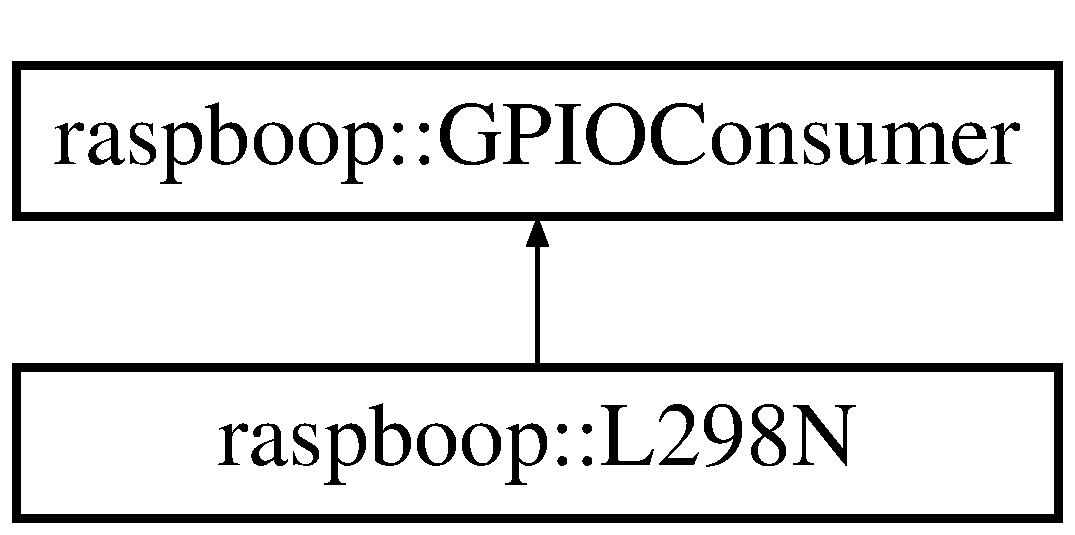
\includegraphics[height=2.000000cm]{classraspboop_1_1L298N}
\end{center}
\end{figure}
\subsection*{Public Member Functions}
\begin{DoxyCompactItemize}
\item 
void \hyperlink{classraspboop_1_1L298N_a02313609416e301b2d9591ec1032c7e6}{Use\-Soft\-P\-W\-M} ()
\begin{DoxyCompactList}\small\item\em Sets the input pins to software P\-W\-M mode. \end{DoxyCompactList}\item 
void \hyperlink{classraspboop_1_1L298N_a0db4bc15c28818ed54e80f65f9f25d72}{Set\-P\-W\-M\-Value} (int I\-N, int Value)
\begin{DoxyCompactList}\small\item\em Sets a pin's software P\-W\-M value. \end{DoxyCompactList}\item 
void \hyperlink{classraspboop_1_1L298N_a18137a4b8e3ba274cf6bf72e896f7563}{Set\-Pin\-Value} (int I\-N, int Value)
\begin{DoxyCompactList}\small\item\em Set a pin's value to either H\-I\-G\-H or L\-O\-W. \end{DoxyCompactList}\item 
virtual void \hyperlink{classraspboop_1_1L298N_a5ed5847ed8db5835fbf5e4f960a374e9}{Release\-Pins} ()
\begin{DoxyCompactList}\small\item\em Sets the mode of all pins to an inactive state. \end{DoxyCompactList}\end{DoxyCompactItemize}
\subsection*{Static Public Member Functions}
\begin{DoxyCompactItemize}
\item 
static \hyperlink{classraspboop_1_1L298N}{L298\-N} $\ast$ \hyperlink{classraspboop_1_1L298N_a57ef1c025baf2584f326722196c1a35b}{Create} (int I\-N1, int I\-N2, int I\-N3, int I\-N4)
\begin{DoxyCompactList}\small\item\em Creates a pointer to an \hyperlink{classraspboop_1_1L298N}{L298\-N} object. \end{DoxyCompactList}\end{DoxyCompactItemize}
\subsection*{Additional Inherited Members}


\subsection{Detailed Description}
\hyperlink{classraspboop_1_1L298N}{L298\-N} Motor controller. 

This class is meant to support the \hyperlink{classraspboop_1_1L298N}{L298\-N} motor controller board. In most cases, the Enable A, B, and 5\-V pins are connected by default through jumpers on most model \#236 board.

\subsection*{Helpful information }


\begin{DoxyItemize}
\item This board is able to control two motors at the same time.
\item Do not input a voltage into the 5\-V terminal
\begin{DoxyItemize}
\item If the voltage in the 12\-V terminal is greater than 12\-V, then you can use the 5\-V terminal as a power source.
\end{DoxyItemize}
\end{DoxyItemize}

\begin{TabularC}{2}
\hline
\rowcolor{lightgray}{\bf Quick Stats }&{\bf Value  }\\\cline{1-2}
Maximum input voltage &{\bfseries 46\-V} \\\cline{1-2}
Continuous output current &{\bfseries 2 Amps} \\\cline{1-2}
Maximum output current &{\bfseries 3 Amps} \\\cline{1-2}
Logical voltage &{\bfseries 5\-V} \\\cline{1-2}
Max Logical current &{\bfseries 36 m\-A} \\\cline{1-2}
Maximum output &{\bfseries 25 W} \\\cline{1-2}
\end{TabularC}
\subsubsection*{External links }

\href{http://www.st.com/st-web-ui/static/active/en/
 resource/technical/document/datasheet/CD00000240.pdf}{\tt Datasheet}

\href{http://zapterra.com/systems/articles/electronics/
 l298-motor-driver-tutorial-arduino/}{\tt Blog post\-:} Very informative and detailed blog post. Recommended if you need an introduction to the chip. 

\subsection{Member Function Documentation}
\hypertarget{classraspboop_1_1L298N_a57ef1c025baf2584f326722196c1a35b}{\index{raspboop\-::\-L298\-N@{raspboop\-::\-L298\-N}!Create@{Create}}
\index{Create@{Create}!raspboop::L298N@{raspboop\-::\-L298\-N}}
\subsubsection[{Create}]{\setlength{\rightskip}{0pt plus 5cm}{\bf L298\-N} $\ast$ raspboop\-::\-L298\-N\-::\-Create (
\begin{DoxyParamCaption}
\item[{int}]{I\-N1, }
\item[{int}]{I\-N2, }
\item[{int}]{I\-N3, }
\item[{int}]{I\-N4}
\end{DoxyParamCaption}
)\hspace{0.3cm}{\ttfamily [static]}}}\label{classraspboop_1_1L298N_a57ef1c025baf2584f326722196c1a35b}


Creates a pointer to an \hyperlink{classraspboop_1_1L298N}{L298\-N} object. 

To properly create an object in raspboop, you must use its factory \hyperlink{classraspboop_1_1L298N_a57ef1c025baf2584f326722196c1a35b}{Create()} method. The factory method initializes the \hyperlink{classraspboop_1_1L298N}{L298\-N}'s pins using the \hyperlink{classraspboop_1_1GPIOConsumer_a066938a39a4f34ed2cfee05a593008e6}{Consume\-Pin()} method.


\begin{DoxyParams}{Parameters}
{\em I\-N1} & The board's I\-N1 pin \\
\hline
{\em I\-N2} & The board's I\-N2 pin \\
\hline
{\em I\-N3} & The board's I\-N3 pin \\
\hline
{\em I\-N4} & The board's I\-N4 pin\\
\hline
\end{DoxyParams}
\begin{DoxyReturn}{Returns}
A pointer to an \hyperlink{classraspboop_1_1L298N}{L298\-N} object with all pins ready to operate. 
\end{DoxyReturn}
\hypertarget{classraspboop_1_1L298N_a5ed5847ed8db5835fbf5e4f960a374e9}{\index{raspboop\-::\-L298\-N@{raspboop\-::\-L298\-N}!Release\-Pins@{Release\-Pins}}
\index{Release\-Pins@{Release\-Pins}!raspboop::L298N@{raspboop\-::\-L298\-N}}
\subsubsection[{Release\-Pins}]{\setlength{\rightskip}{0pt plus 5cm}void raspboop\-::\-L298\-N\-::\-Release\-Pins (
\begin{DoxyParamCaption}
{}
\end{DoxyParamCaption}
)\hspace{0.3cm}{\ttfamily [virtual]}}}\label{classraspboop_1_1L298N_a5ed5847ed8db5835fbf5e4f960a374e9}


Sets the mode of all pins to an inactive state. 

All children must call this method when it becomes out of scope, preferably in the destructor. This is necessary so that there are never any G\-P\-I\-O pins unnecessarily set to {\itshape H\-I\-G\-H} 

Implements \hyperlink{classraspboop_1_1GPIOConsumer_a97b06b9afddfb338fb87cb7338c910de}{raspboop\-::\-G\-P\-I\-O\-Consumer}.

\hypertarget{classraspboop_1_1L298N_a18137a4b8e3ba274cf6bf72e896f7563}{\index{raspboop\-::\-L298\-N@{raspboop\-::\-L298\-N}!Set\-Pin\-Value@{Set\-Pin\-Value}}
\index{Set\-Pin\-Value@{Set\-Pin\-Value}!raspboop::L298N@{raspboop\-::\-L298\-N}}
\subsubsection[{Set\-Pin\-Value}]{\setlength{\rightskip}{0pt plus 5cm}void raspboop\-::\-L298\-N\-::\-Set\-Pin\-Value (
\begin{DoxyParamCaption}
\item[{int}]{I\-N, }
\item[{int}]{Value}
\end{DoxyParamCaption}
)}}\label{classraspboop_1_1L298N_a18137a4b8e3ba274cf6bf72e896f7563}


Set a pin's value to either H\-I\-G\-H or L\-O\-W. 

This is equivalent to calling wiring\-Pi's digital\-Write() method


\begin{DoxyParams}{Parameters}
{\em I\-N} & Value of 1 $\sim$ 4 that represents the physical I\-N pin on the board \\
\hline
{\em Value} & A value of H\-I\-G\-H(1) or L\-O\-W(0) \\
\hline
\end{DoxyParams}
\hypertarget{classraspboop_1_1L298N_a0db4bc15c28818ed54e80f65f9f25d72}{\index{raspboop\-::\-L298\-N@{raspboop\-::\-L298\-N}!Set\-P\-W\-M\-Value@{Set\-P\-W\-M\-Value}}
\index{Set\-P\-W\-M\-Value@{Set\-P\-W\-M\-Value}!raspboop::L298N@{raspboop\-::\-L298\-N}}
\subsubsection[{Set\-P\-W\-M\-Value}]{\setlength{\rightskip}{0pt plus 5cm}void raspboop\-::\-L298\-N\-::\-Set\-P\-W\-M\-Value (
\begin{DoxyParamCaption}
\item[{int}]{I\-N, }
\item[{int}]{Value}
\end{DoxyParamCaption}
)}}\label{classraspboop_1_1L298N_a0db4bc15c28818ed54e80f65f9f25d72}


Sets a pin's software P\-W\-M value. 

This method uses wiring\-Pi's \href{http://wiringpi.com/reference/
software-pwm-library/}{\tt software P\-W\-M library} to set the software P\-W\-M on the pin to a value. You must first call the Use\-Soft\-Pwm() method before using this method.


\begin{DoxyParams}{Parameters}
{\em I\-N} & Value of 1 $\sim$ 4 that represents the physical I\-N pin on the board \\
\hline
{\em Value} & A value from 0 to 100 \\
\hline
\end{DoxyParams}
\hypertarget{classraspboop_1_1L298N_a02313609416e301b2d9591ec1032c7e6}{\index{raspboop\-::\-L298\-N@{raspboop\-::\-L298\-N}!Use\-Soft\-P\-W\-M@{Use\-Soft\-P\-W\-M}}
\index{Use\-Soft\-P\-W\-M@{Use\-Soft\-P\-W\-M}!raspboop::L298N@{raspboop\-::\-L298\-N}}
\subsubsection[{Use\-Soft\-P\-W\-M}]{\setlength{\rightskip}{0pt plus 5cm}void raspboop\-::\-L298\-N\-::\-Use\-Soft\-P\-W\-M (
\begin{DoxyParamCaption}
{}
\end{DoxyParamCaption}
)}}\label{classraspboop_1_1L298N_a02313609416e301b2d9591ec1032c7e6}


Sets the input pins to software P\-W\-M mode. 

Uses wiring\-Pi's \href{http://wiringpi.com/
reference/software-pwm-library/}{\tt software P\-W\-M library} to set the pins provided in the \hyperlink{classraspboop_1_1L298N_a57ef1c025baf2584f326722196c1a35b}{Create()} factory method to a software P\-W\-M mode

{\bfseries Note\-:} Software P\-W\-M operates on seperate threads, and each thread consumes about 0.\-5\% C\-P\-U, according to the wiring\-Pi reference. 

The documentation for this class was generated from the following files\-:\begin{DoxyCompactItemize}
\item 
include/raspboop/boards/L298\-N.\-h\item 
src/boards/L298\-N.\-cpp\end{DoxyCompactItemize}

\hypertarget{classraspboop_1_1Sensor}{\section{raspboop\-:\-:Sensor Class Reference}
\label{classraspboop_1_1Sensor}\index{raspboop\-::\-Sensor@{raspboop\-::\-Sensor}}
}


An abstract class for devices that can interface with the world.  




{\ttfamily \#include $<$Sensor.\-h$>$}

Inheritance diagram for raspboop\-:\-:Sensor\-:\begin{figure}[H]
\begin{center}
\leavevmode
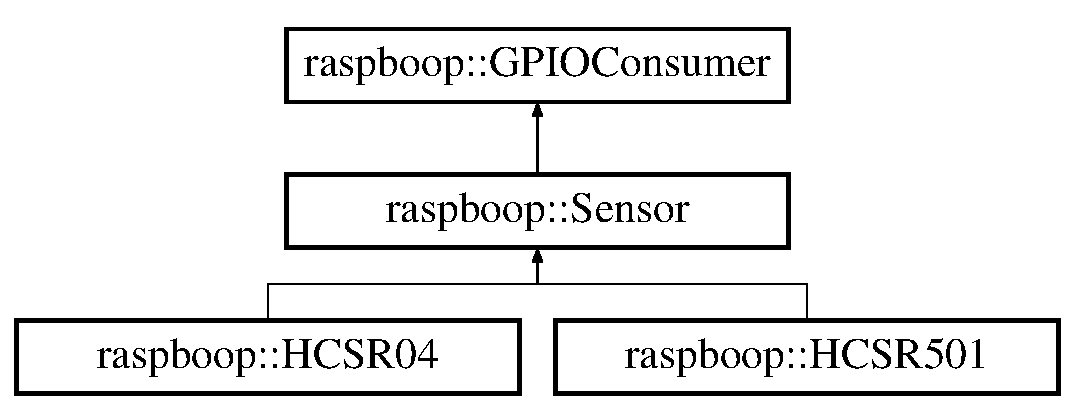
\includegraphics[height=3.000000cm]{classraspboop_1_1Sensor}
\end{center}
\end{figure}
\subsection*{Public Member Functions}
\begin{DoxyCompactItemize}
\item 
virtual void \hyperlink{classraspboop_1_1Sensor_ab854a10682373803a310c078bb71aacf}{Sense} ()=0
\begin{DoxyCompactList}\small\item\em Performs the sensor's sensing operation. \end{DoxyCompactList}\end{DoxyCompactItemize}
\subsection*{Protected Member Functions}
\begin{DoxyCompactItemize}
\item 
void \hyperlink{classraspboop_1_1Sensor_a893f7ad09018028fdb9e10f0bcbeccf9}{Set\-Output\-Pin} (int Pin)
\begin{DoxyCompactList}\small\item\em Set an output pin for the sensor. \end{DoxyCompactList}\item 
void \hyperlink{classraspboop_1_1Sensor_ad0b3f0fa153803108613e3c3da574571}{Set\-Input\-Pin} (int Pin)
\begin{DoxyCompactList}\small\item\em Set an input pin for the sensor. \end{DoxyCompactList}\end{DoxyCompactItemize}


\subsection{Detailed Description}
An abstract class for devices that can interface with the world. 

Sensors can sense the world and provide valuable data about the state of the current environment.

Most sensors require an output, or a trigger, G\-P\-I\-O pin that tells the sensor when to sense. An example of this type of sensor is the \hyperlink{classraspboop_1_1HCSR04}{H\-C\-S\-R04} ultrasonic distance sensor. However, there are sensors that persistently report its value back to a G\-P\-I\-O pin. An example of this type of sensor is the \hyperlink{classraspboop_1_1HCSR501}{H\-C\-S\-R501} passive infrared sensor.

In both cases, there is a need for either an output pin and/or an input pin. 

\subsection{Member Function Documentation}
\hypertarget{classraspboop_1_1Sensor_ab854a10682373803a310c078bb71aacf}{\index{raspboop\-::\-Sensor@{raspboop\-::\-Sensor}!Sense@{Sense}}
\index{Sense@{Sense}!raspboop::Sensor@{raspboop\-::\-Sensor}}
\subsubsection[{Sense}]{\setlength{\rightskip}{0pt plus 5cm}virtual void raspboop\-::\-Sensor\-::\-Sense (
\begin{DoxyParamCaption}
{}
\end{DoxyParamCaption}
)\hspace{0.3cm}{\ttfamily [pure virtual]}}}\label{classraspboop_1_1Sensor_ab854a10682373803a310c078bb71aacf}


Performs the sensor's sensing operation. 

This method will retrieve a value from the environment by performing G\-P\-I\-O operations on the input and output pins of the sensor. The value from the sensor will be available through an accessor method. 

Implemented in \hyperlink{classraspboop_1_1HCSR04_ab25ac4ca02a3a3e3b00d0df95c58f447}{raspboop\-::\-H\-C\-S\-R04}, and \hyperlink{classraspboop_1_1HCSR501_ade0ae21c1bda3dabec68e0476d92520a}{raspboop\-::\-H\-C\-S\-R501}.

\hypertarget{classraspboop_1_1Sensor_ad0b3f0fa153803108613e3c3da574571}{\index{raspboop\-::\-Sensor@{raspboop\-::\-Sensor}!Set\-Input\-Pin@{Set\-Input\-Pin}}
\index{Set\-Input\-Pin@{Set\-Input\-Pin}!raspboop::Sensor@{raspboop\-::\-Sensor}}
\subsubsection[{Set\-Input\-Pin}]{\setlength{\rightskip}{0pt plus 5cm}void raspboop\-::\-Sensor\-::\-Set\-Input\-Pin (
\begin{DoxyParamCaption}
\item[{int}]{Pin}
\end{DoxyParamCaption}
)\hspace{0.3cm}{\ttfamily [protected]}}}\label{classraspboop_1_1Sensor_ad0b3f0fa153803108613e3c3da574571}


Set an input pin for the sensor. 

Consumes a pin to be designated as an input. This is usually the pin that will be receiving data from the sensor.


\begin{DoxyParams}{Parameters}
{\em Pin} & The pin to designate as in input \\
\hline
\end{DoxyParams}
\hypertarget{classraspboop_1_1Sensor_a893f7ad09018028fdb9e10f0bcbeccf9}{\index{raspboop\-::\-Sensor@{raspboop\-::\-Sensor}!Set\-Output\-Pin@{Set\-Output\-Pin}}
\index{Set\-Output\-Pin@{Set\-Output\-Pin}!raspboop::Sensor@{raspboop\-::\-Sensor}}
\subsubsection[{Set\-Output\-Pin}]{\setlength{\rightskip}{0pt plus 5cm}void raspboop\-::\-Sensor\-::\-Set\-Output\-Pin (
\begin{DoxyParamCaption}
\item[{int}]{Pin}
\end{DoxyParamCaption}
)\hspace{0.3cm}{\ttfamily [protected]}}}\label{classraspboop_1_1Sensor_a893f7ad09018028fdb9e10f0bcbeccf9}


Set an output pin for the sensor. 

Consumes a pin to be designated as an output. This is usually the pin that triggers sensing.


\begin{DoxyParams}{Parameters}
{\em Pin} & The pin to designate as an output \\
\hline
\end{DoxyParams}


The documentation for this class was generated from the following files\-:\begin{DoxyCompactItemize}
\item 
include/raspboop/abstracts/Sensor.\-h\item 
src/abstracts/Sensor.\-cpp\end{DoxyCompactItemize}

%--- End generated contents ---

% Index
\newpage
\phantomsection
\addcontentsline{toc}{chapter}{Index}
\printindex

\end{document}
